\section{Reducibility and Hardness}
\label{sec:reduce-and-hard}

You many already know that we can map some problems onto other problems. In
fact, we did this in the previous example with \texttt{2-SAT}, where we mapped
it onto a graph pathfinding problem.

It turns out that mapping problems onto other problems can be well defined
theoretically. if one problem $P_1$ can be mapped onto $P_2$, then we say that
$P_1$ is many-one-logspace reducible to $P_2$.

Formally, let $P_1$ be over the alphabet $\Sigma_a$, and $P_2$ be over the
alphabet $\Sigma_b$. $P_1$ is reducible to $P_2$ if there exists a function $f :
\Sigma^*_a \rightarrow \Sigma^*_b$ that is in \texttt{SPACE(log n)}, such that
$x \in \Sigma^*_a,~x \in P_1~\text{iff}~f(x)\in P_2$.

In English, this is saying that a problem is reducible to another problem if we
can make a function that runs in $log(n)$ space, that converts all instances of
the first problem into an equivalent instance of the second problem.

The notation for reducibility is:

\marginpar{This is also called a many-one logspace reduction.}

\[
  P_1 \leq^{log}_m P_2
\]

Reducibility is helpful for a number of reasons:

\begin{itemize}
  \item If $P_1 \leq^{log}_m P_2$, then $P_2$ is at least as hard as $P_1$.
  \item Similarly, $P_1$ is no harder than $P_2$.
  \item If anybody comes up with a way of solving $P_2$ fast, then we can use 
    the same way to solve $P_1$.
  \marginpar{This only works for some (most) complexity classes, e.g.
    \texttt{LogSpace}, \texttt{NLogSpace}, \texttt{PTime}, \texttt{NPTime}.
    Not \texttt{Time(n)} or \texttt{Time(}$n^2$\texttt{)}.}
  \item \textbf{We can use reducibility to show that a problem is inside a 
    complexity class by reducing it to one that you know is in the desired
    class.}
\end{itemize}

Reducibility is transitive, so if $P_1 \leq^{log}_m P_2$ and $P_2 \leq^{log}_m P_3$, then $P_1 \leq^{log}_m P_3$. The reason why, is that if:

\[
  f_1 : \Sigma^*_{P_1} \rightarrow \Sigma^*_{P_2}
\]
\[
  f_2 : \Sigma^*_{P_2} \rightarrow \Sigma^*_{P_3}
\]

We have a Turing Machine $M$ that can compute a function $f_3 = f_2 \cdot f_1$,
which essentially is:

\[
  f_3 : \Sigma^*_{P_1} \rightarrow \Sigma^*_{P_3}
\]

Lets define $M$:

\begin{lstlisting}[numbers=left,mathescape]
  Calculate the first bit of $f_1(x)$
  Keep a counter to say what bit we've calculated ($1$ at first)
  Start a simulation of $f_2(f_1(x))$, where the argument is the calculated bit
  If $f_2$ asks to move the read head right:
    Calculate the next bit of $f_1(x)$
    Write it on top of the current bit
    Update the output bit counter
  Else, if $f_2$ asks to move the read head left:
    Restart the calculation of $f_1(x)$
    Continue calculating until we have the desired output bit
    Write it on top of the current bit
    Update the bit counter
\end{lstlisting}

Although $M$ horrifies my programmer-mind at how inefficient it is, I conclude
that it does in fact run in logarithmic space (it seems to run in constant space
at first, but then you realise that the counter requires $log_2(n)$ bits, and
that the functions its emulating, $f_1$ and $f_2$, run in log space).

A \textit{many-one polytime} reduction is a weaker notion of reducibility where
instead of a function that runs in log space to convert the strings of one
problem into the strings of another, we have one that is in \texttt{TIME\{P\}}
instead. If this is the case, then the reducibility is mathematically written
as:

\[
  P_1 \leq_m^P P_2
\]

\marginpar{Many-one polynomial reducibility is transitive because any 
polynomial multiplied by any other polynomial is still a polynomial.}

However, \textit{many-one logspace} reducibility trumps its polynomial cousin,
since while they're both transitive, the former is theoretically a bit more
useful, and many polytime reduciblities are in fact logspace ones.

A problem $P \in X$ is said to be \textit{X}-\textbf{complete}, when $X$ is a
complexity class, when for all problem $Q \in X$, $Q \leq_m^{log} P$. This means
that $P$ is at least as hard as all problems $X$.

If $P \notin X$, then $P$ is not \textit{X}-complete, but is
\textit{X}-\textbf{hard}.

\subsection{Cook's theorem}

The Cook Levin theorem proves that \texttt{SAT} is \texttt{NPTime-Complete}.
This is important, because certain interesting problems were shown to be
\texttt{NP-Complete}, and if any of these problems are solved in
(deterministic) polynomial time, then all of the problems would be solvable in
polynomial time.

The idea behind the Cook Levin theorem, is to turn any Turing Machine $M$ that
solves a problem $P$ into a set of clauses that can be solved by \texttt{SAT},
and we can do this in deterministic polynomial time. If we can solve
\texttt{SAT} in better-than \texttt{NPTime}, then we can solve $P$ in the same
time.

We can also show that \texttt{3-SAT} is \texttt{NP-Complete}. Obviously
\texttt{3-SAT} $\in$ \texttt{SAT}, but to prove completeness, we need to show
that every problem in \texttt{SAT} can be converted to a problem in
\texttt{3-SAT}. We can use the following rules:

\begin{itemize}
  \item For each input clause of length 1:
    $\{a\} \rightarrow \{a \vee a \vee a\}$ 
  \item For each input clause of length 2:
    $\{a \vee b\} \rightarrow \{a \vee b \vee a\}$ 
  \item For each input clause of length 3, do nothing!
  \item For each input clause of length $n \geq 3$:
    $\{a \vee b \vee c \vee d \vee e\} \rightarrow
      \{a \vee b \vee x\},
      \{\neg x \vee c \vee y\},
      \{\neg y \vee d \vee e\}$ 
\end{itemize}

Hence \texttt{3-SAT} is \texttt{NP-Complete}. Similarly, we can reduce
\texttt{3-SAT} to the $0/1$ Integer Linear Programming problem and hence (since
we know it's in \texttt{NP-Time}) prove that ILP is \texttt{NP-Complete}.

As was said in Section~\ref{sec:ip}, it is possible to do cool stuff with
Integer Programming. In order to convert \texttt{3-SAT} clauses to integer
programming equations we need to:

\begin{itemize}
  \item Make an equation for each literal $x$ such that $l_x + l_{\neg x} = 1$,
  so that every literal is either positive or negative.

  \item For every clause $\{a \vee b \vee c\}$ in the input, we make an 
  equation with two new variables ($u,v$) in (unique to the equation):
  $l_a + l_b + l_c + u + v = 3$. Then if the clause is true (so at least one of 
  its literals is true), then we can set $u$ and $v$ to a value that will make 
  the equation hold.
\end{itemize}

\marginpar{N.b., \texttt{NP-Complete} is mostly synonymous with
\texttt{NPTime-Complete}.}

If we then solve the ILP programming problem for these equations, then we can
find a suitable truth assignment for \texttt{3-SAT}, and so we have proved that
\texttt{ILP(0/1)} is \texttt{NPTime-Complete}.

\subsection{3-SAT as a graph colouring problem}
\label{sat-colour}

We can show that \textit{3-colourability} is \texttt{NP-Time} hard, because we
can convert an instance of \texttt{3-SAT} into it. Given a \texttt{3-SAT}
problem, we compute in log space (since we want a many-one log reduction), a
function to create a graph from the satisfiability problem's clauses.

To do this, we create three `gadgets' which let us represent logical gates in
graph form. The gadgets have internal nodes which make them easier to draw, the
internal nodes are not often shown in larger sketches, but are when describing
the gadgets initially in order to make the properties of the gadget known.

\begin{description}
  \item \textbf{Gadget 1: Equality}\\
    We want to make a gadget that will make sure that two nodes have the same 
    colour. Here, $a$ and $b$ are the input and output nodes, while the other 
    two nodes are internal. In any $3$ colouring, $a$ and $b$ must be the same  
    colour:

    \begin{figure}[H]
      \centering
      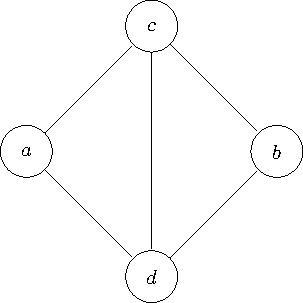
\includegraphics[width=0.4\textwidth]{diagrams/graph11}
      \caption{Gadget 1}
      \label{fig:gadget1}
    \end{figure}

  \item \textbf{Gadget 2: XOR Gate}\\
    I'm not sure if this is strictly an XOR gate, but that's what it reminds me 
    of. $a$ is either the same colour as $b$ or $c$, while $d$ is an internal 
    node.

    \begin{figure}[H]
      \centering
      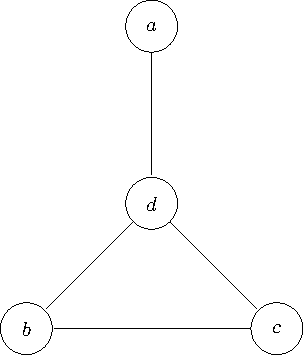
\includegraphics[width=0.4\textwidth]{diagrams/graph12}
      \caption{Gadget 2}
      \label{fig:gadget2}
    \end{figure}

    Note that we can chain this gadget like a normal XOR gate if we attach
    another Gadget 2 to the $c$ node. Then $a$ will have the same colour as $b$,
    or the one of the children of the second gadget.

  \item \textbf{Gadget 3: OR Gate}\\
    This gadget has lots of nodes, though again, only $a$, $b$ and $c$ are 
    external. Now, $a$ is the same as either $b$, or $c$, or both $b$ and $c$.

    \begin{figure}[H]
      \centering
      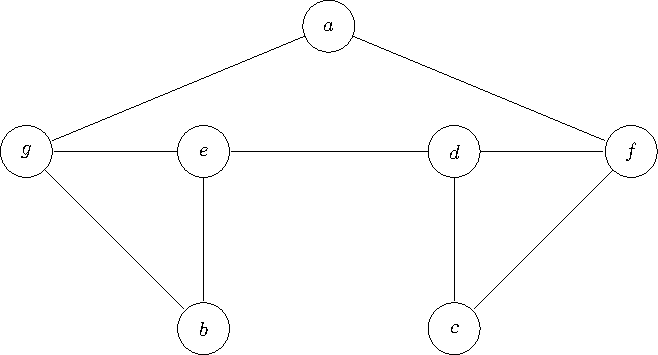
\includegraphics[width=0.4\textwidth]{diagrams/graph13}
      \caption{Gadget 3}
      \label{fig:gadget3}
    \end{figure}
\end{description}

I tried to encode $(a \vee \neg b), (b \vee c)$ as a colourability problem (shown
in Figure~\ref{fig:k-color-3-sat}) but I did it wrong\dots Since it takes so
long to write the graphs in \LaTeX, I thought I'd let you spot the mistake I
made ;)

\begin{figure}[H]
  \centering
  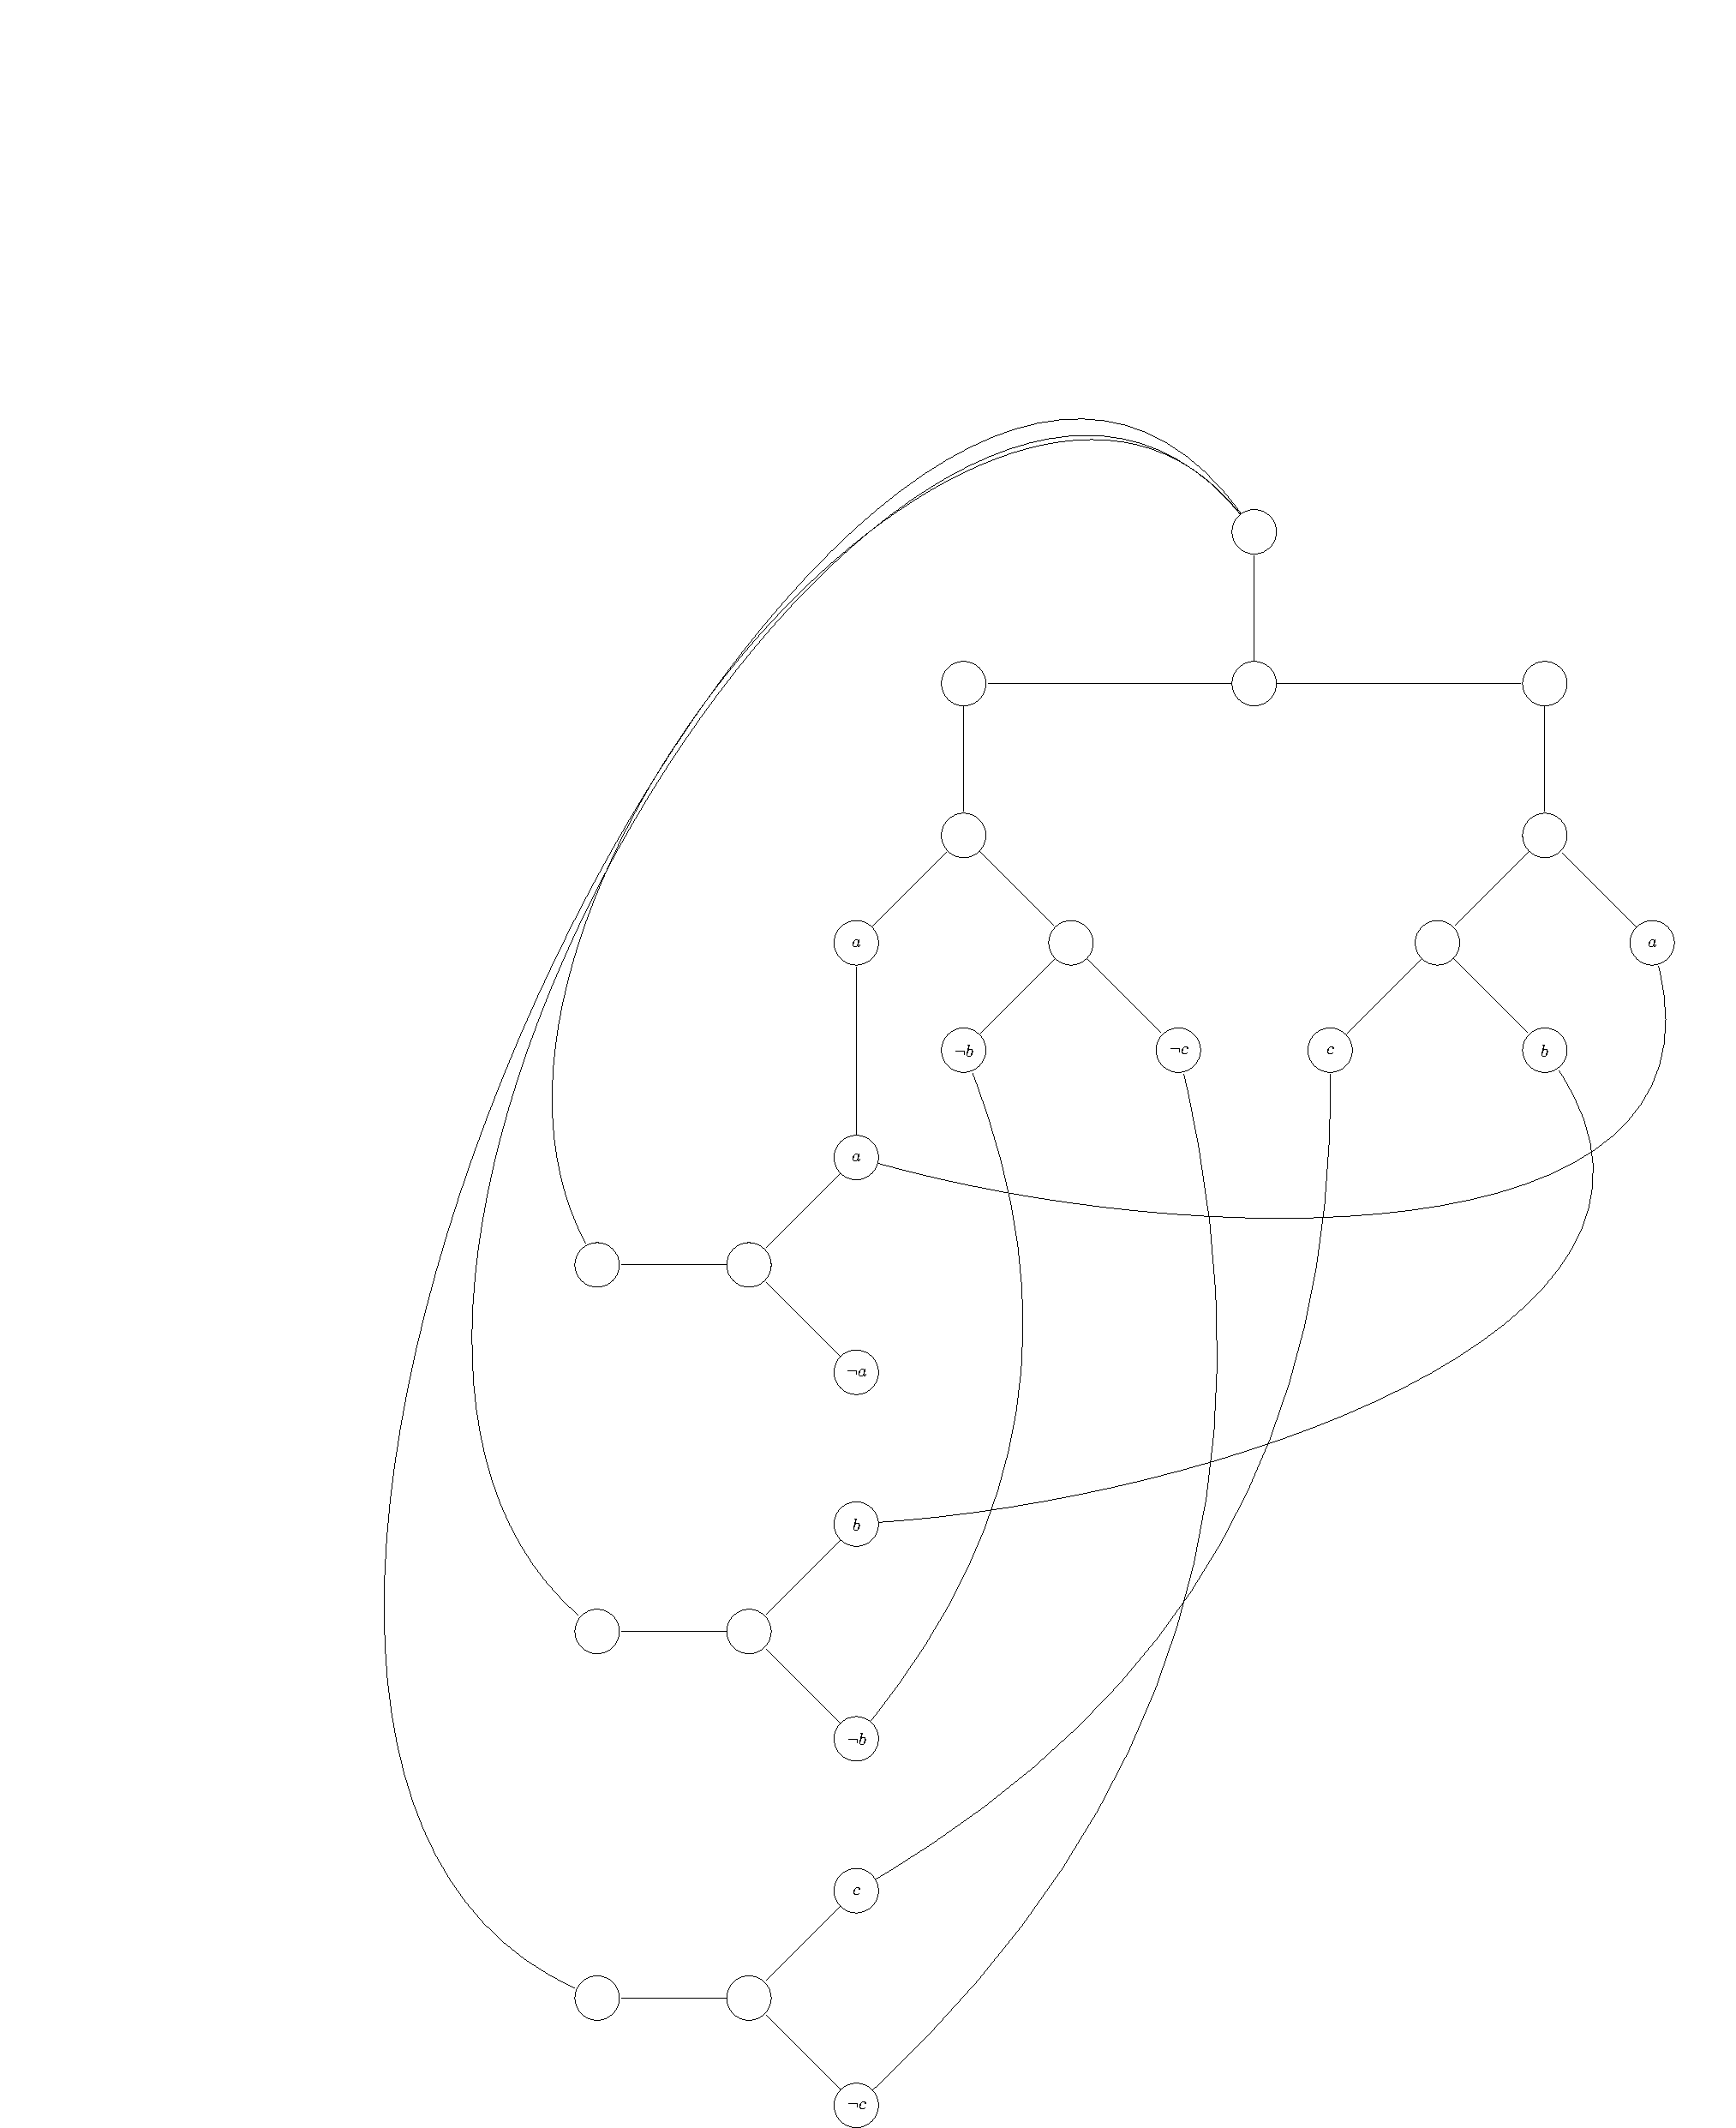
\includegraphics[width=\textwidth]{diagrams/graph14}
  \caption{An incorrect encoding in \textit{k-colourability} of the \texttt{SAT} 
  problem $(a \vee \neg b), (b \vee c)$. The problem is that I used the wrong
  gadget (I used the second one instead of the third one) for the top row of
  nodes. Also, I've encoded a \texttt{SAT} problem, not a \texttt{3-SAT} problem
  so that's not really right either. Feel free to fix this with a pull request!}
  \label{fig:k-colour-3-sat}
\end{figure}

\subsection{Space complexity}

\marginpar{Make sure you read over lectures 10 and 11; there's a lot of stuff 
I've not included here.}

Just like time complexity, space complexity is also measured using the Big-Oh
notation. \texttt{Space(f(n))} is the space (number of tape cells) used by a
deterministic Turing Machine, and \texttt{NSpace(f(n))} is the same for a
nondeterministic Turing Machine.

Savich's theorem describes the relationship between deterministic and non-
deterministic space complexity. We know that we can make a deterministic TM
simulate a non-deterministic one in exponential time by simulating all branches
of the latter's computation tree. Savich's theorem shows that a deterministic TM
can simulate a non-deterministic one in the square of the space that would
normally be used:

\marginpar{What does the Computer Scientist say when he goes into space?
``OMG, $P = NP$!''}

\[
  NSpace(f(n)) \in Space(f^2(n))
\]

This is demonstrated by using directed graph reachability as an example. Given
the directed graph $G$, we can determine if one node is reachable from another
using an algorithm like:

\begin{lstlisting}[language=python]
  # For log
  import math

  graph = {0 : [1,3,4],
           1 : [0,2],
           2 : [1,3],
           3 : [0,2],
           4 : [0]}

  def is_reachable(start, end, graph, steps):
    print "is_reachable(%d, %d, graph, %d)" % (start, end, steps)
    if steps == 0:
      return start == end or (end in graph[start])
    else:
      for adj in graph[start]:
        if is_reachable(start, adj, graph, steps - 1):
          if is_reachable(adj, end, graph, steps - 1):
            return True
      return False

  print is_reachable(0, 3, graph, int(math.log(len(graph), 2))) # True
  print is_reachable(4, 2, graph, int(math.log(len(graph), 2))) # False
\end{lstlisting}

\texttt{is\_reachable} finds if there is a path between the start and end nodes
within $2^{steps}$ steps. In order to find if the nodes are connected in the
graph, we have to give it $log_2(|graph|)$ as the steps parameter. This works
because any path from $start$ to $end$ in $2^x$ steps must have a midpoint
$mid$. If we find a path from $start$ to $mid$ in $2^{x - 1}$ steps, and a path
from $mid$ to $end$ in the same number, then we'll can put them together and
find the complete path.

On a Turing Machine, we implement this by writing a tuple
\texttt{(start,end,steps)} to the work tape on every step of the recursion. This
requires $O(h \times log_2(|V|))$ space, and since we set $steps$ to be $log_2
(|graph|)$, the total space complexity is $O(log_2(|V|) \times log_2(|V|)) = O(
log^2_2(|V|))$.

We can generalise this to any TM; if we visualise the execution of a non-
deterministic TM as a graph, we can use the reachability algorithm above to
determine whether we can reach an accepting state from the start state and we
can do it in $SPACE(O(f(n))^2)$. This gives the result that $NSpace(f(n)) \in
Space(f^2(n))$.

We can solve directed reachability with a depth first search in deterministic
linear time and space, and have just shown that we can use
\texttt{num\_reachability} to solve it in $Space(log(n)^2)$, but we can in fact
do even better space-wise.
